\documentclass{article}
% translate with >> pdflatex -shell-escape <file>

% This file is used as unit test for pgfplots, copyright by Christian Feuersaenger.
% 
% See
%   http://pgfplots.sourceforge.net/pgfplots.pdf
% for pgfplots.
%
% Any required input files (for <plot table> or <plot file> or the table package) can be downloaded
% at
% http://www.ctan.org/tex-archive/graphics/pgf/contrib/pgfplots/doc/latex/
% and
% http://www.ctan.org/tex-archive/graphics/pgf/contrib/pgfplots/doc/latex/plotdata/

\usepackage{pgfplots}
\usepackage{pgfplotstable}
\pgfplotsset{compat=1.4}

\pagestyle{empty}

\begin{document}

\pgfplotsset{
	view={0}{90},
	error bars/.cd,
	y dir=both,
	y explicit,
	x dir=both,
	x explicit,
	error bar style={black,dotted,error bars/error mark=square*,error bars/error mark options={current plot style}},
}

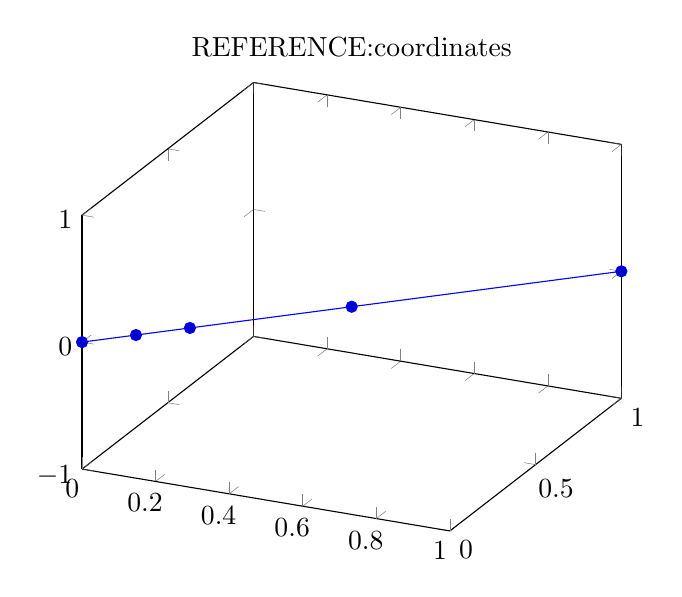
\begin{tikzpicture}
\begin{axis}[title={REFERENCE:coordinates}]
\addplot3+[
]
	coordinates
	{(0,0,0) +- (0.5,0.1,0) 
	(0.1,0.1,0)  +- (0.05,0.2,0)
	(0.2,0.2,0) 	+- (0,0.05,0)
	(0.5,0.5,0) +- (0.1,0.2,0)
	(1,1,0) +- (0.3,0.1,0)
	};
\end{axis}
\end{tikzpicture}

%\tracingmacros=2 \tracingcommands=2

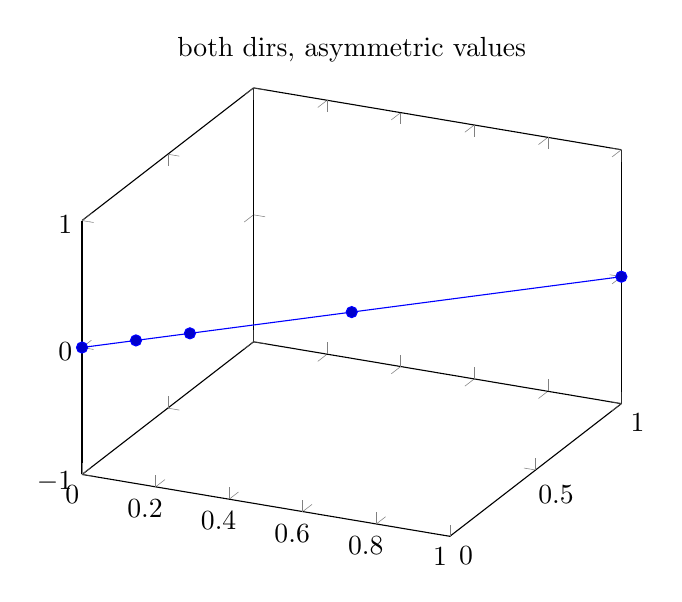
\begin{tikzpicture}
\begin{axis}[title={both dirs, asymmetric values},]
\addplot3+[
]
	coordinates
	{(0,0,0) += (0.5,0.1,0)  -= (0.1,0.05,0)
	(0.1,0.1,0)  += (0.05,0.2,0) -= (0,0,0)
	(0.2,0.2,0) 	+= (0,0.05,0) -= (1,0.2,0)
	(0.5,0.5,0) += (0.1,0.2,0) -= (0.2,0.1,0)
	(1,1,0) +- (0.3,0.1,0)
	};
\end{axis}
\end{tikzpicture}
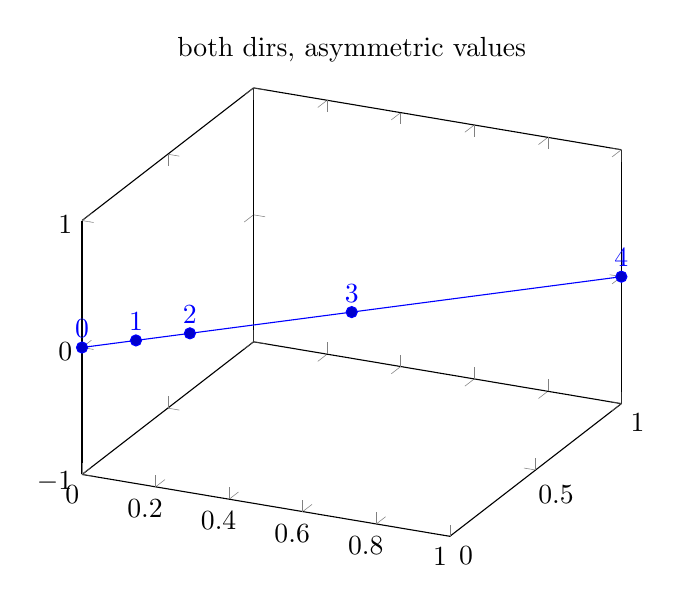
\begin{tikzpicture}
\begin{axis}[title={both dirs, asymmetric values},nodes near coords]
\addplot3+[
	point meta=explicit,
]
	coordinates
	{(0,0,0) += (0.5,0.1,0)  -= (0.1,0.05,0) [0]
	(0.1,0.1,0)  += (0.05,0.2,0) -= (0,0,0)  [1]
	(0.2,0.2,0) 	+= (0,0.05,0) -= (1,0.2,0) [2]
	(0.5,0.5,0) += (0.1,0.2,0) -= (0.2,0.1,0) [3]
	(1,1,0) +- (0.3,0.1,0) [4]
	};
\end{axis}
\end{tikzpicture}
\end{document}
